
\documentclass[12pt]{article}
%\usepackage[finnish]{babel}
\usepackage[T1]{fontenc}
\usepackage[utf8]{inputenc}
\usepackage{delarray,amsmath,bbm,epsfig,slashed}
\usepackage{bbold}
\usepackage{listings}
\usepackage{qcircuit}
\usepackage{graphicx}
\newcommand{\pat}{\partial}
\newcommand{\be}{\begin{equation}}
\newcommand{\ee}{\end{equation}}
\newcommand{\bea}{\begin{eqnarray}}
\newcommand{\eea}{\end{eqnarray}}
\newcommand{\abf}{{\bf a}}
\newcommand{\Zmath}{\mathbf{Z}}
\newcommand{\Zcal}{{\cal Z}_{12}}
\newcommand{\zcal}{z_{12}}
\newcommand{\Acal}{{\cal A}}
\newcommand{\Fcal}{{\cal F}}
\newcommand{\Ucal}{{\cal U}}
\newcommand{\Vcal}{{\cal V}}
\newcommand{\Ocal}{{\cal O}}
\newcommand{\Rcal}{{\cal R}}
\newcommand{\Scal}{{\cal S}}
\newcommand{\Lcal}{{\cal L}}
\newcommand{\Hcal}{{\cal H}}
\newcommand{\hsf}{{\sf h}}
\newcommand{\half}{\frac{1}{2}}
\newcommand{\Xbar}{\bar{X}}
\newcommand{\xibar}{\bar{\xi }}
\newcommand{\barh}{\bar{h}}
\newcommand{\Ubar}{\bar{\cal U}}
\newcommand{\Vbar}{\bar{\cal V}}
\newcommand{\Fbar}{\bar{F}}
\newcommand{\zbar}{\bar{z}}
\newcommand{\wbar}{\bar{w}}
\newcommand{\zbarhat}{\hat{\bar{z}}}
\newcommand{\wbarhat}{\hat{\bar{w}}}
\newcommand{\wbartilde}{\tilde{\bar{w}}}
\newcommand{\barone}{\bar{1}}
\newcommand{\bartwo}{\bar{2}}
\newcommand{\nbyn}{N \times N}
\newcommand{\repres}{\leftrightarrow}
\newcommand{\Tr}{{\rm Tr}}
\newcommand{\tr}{{\rm tr}}
\newcommand{\ninfty}{N \rightarrow \infty}
\newcommand{\unitk}{{\bf 1}_k}
\newcommand{\unitm}{{\bf 1}}
\newcommand{\zerom}{{\bf 0}}
\newcommand{\unittwo}{{\bf 1}_2}
\newcommand{\holo}{{\cal U}}
%\newcommand{\bra}{\langle}
%\newcommand{\ket}{\rangle}
\newcommand{\muhat}{\hat{\mu}}
\newcommand{\nuhat}{\hat{\nu}}
\newcommand{\rhat}{\hat{r}}
\newcommand{\phat}{\hat{\phi}}
\newcommand{\that}{\hat{t}}
\newcommand{\shat}{\hat{s}}
\newcommand{\zhat}{\hat{z}}
\newcommand{\what}{\hat{w}}
\newcommand{\sgamma}{\sqrt{\gamma}}
\newcommand{\bfE}{{\bf E}}
\newcommand{\bfB}{{\bf B}}
\newcommand{\bfM}{{\bf M}}
\newcommand{\cl} {\cal l}
\newcommand{\ctilde}{\tilde{\chi}}
\newcommand{\ttilde}{\tilde{t}}
\newcommand{\ptilde}{\tilde{\phi}}
\newcommand{\utilde}{\tilde{u}}
\newcommand{\vtilde}{\tilde{v}}
\newcommand{\wtilde}{\tilde{w}}
\newcommand{\ztilde}{\tilde{z}}

% David Weir's macros


\newcommand{\nn}{\nonumber}
\newcommand{\com}[2]{\left[{#1},{#2}\right]}
\newcommand{\mrm}[1] {{\mathrm{#1}}}
\newcommand{\mbf}[1] {{\mathbf{#1}}}
\newcommand{\ave}[1]{\left\langle{#1}\right\rangle}
\newcommand{\halft}{{\textstyle \frac{1}{2}}}
\newcommand{\ie}{{\it i.e.\ }}
\newcommand{\eg}{{\it e.g.\ }}
\newcommand{\cf}{{\it cf.\ }}
\newcommand{\etal}{{\it et al.}}
\newcommand{\ket}[1]{\vert{#1}\rangle}
\newcommand{\bra}[1]{\langle{#1}\vert}
\newcommand{\bs}[1]{\boldsymbol{#1}}
\newcommand{\xv}{{\bs{x}}}
\newcommand{\yv}{{\bs{y}}}
\newcommand{\pv}{{\bs{p}}}
\newcommand{\kv}{{\bs{k}}}
\newcommand{\qv}{{\bs{q}}}
\newcommand{\bv}{{\bs{b}}}
\newcommand{\ev}{{\bs{e}}}
\newcommand{\gv}{\bs{\gamma}}
\newcommand{\lv}{{\bs{\ell}}}
\newcommand{\nabv}{{\bs{\nabla}}}
\newcommand{\sigv}{{\bs{\sigma}}}
\newcommand{\notvec}{\bs{0}_\perp}
\newcommand{\inv}[1]{\frac{1}{#1}}
%\newcommand{\xv}{{\bs{x}}}
%\newcommand{\yv}{{\bs{y}}}
\newcommand{\Av}{\bs{A}}
%\newcommand{\lv}{{\bs{\ell}}}
\newcommand{\Rmath}{\mbf{R}}
\newcommand{\bigzero}{\mbox{\normalfont\Large\bfseries 0}}
\newcommand{\rvline}{\hspace*{-\arraycolsep}\vline\hspace*{-\arraycolsep}}


%\newcommand\bsigma{\vec{\sigma}}
\hoffset 0.5cm
\voffset -0.4cm
\evensidemargin -0.2in
\oddsidemargin -0.2in
\topmargin -0.2in
\textwidth 6.3in
\textheight 8.4in

\begin{document}

\normalsize

\baselineskip 14pt

\begin{center}
{\Large {\bf Quantum Information B \ \ Fall 2020 \ \  Solutions to Problem Set 6}} \\
Jake Muff \\
7/12/20
\end{center}

\bigskip
\section{Answers}

\begin{enumerate}
    \item Exercise 10.38. $U$ and $V$ are unitary operators on two qubits which transform $Z_1, Z_2, X_1, X_2$. Suppose we have a set 
    $$ S = \{ Z_1, Z_2, X_1, X_2 \} $$
    Because $U$ and $V$ is unitary 
    $$ US U^{\dagger} = VSV^{\dagger} $$
    $$ (U^{\dagger} V) S = S (U^{\dagger} V) $$
    As shown in the book for 4x4 matrices 
    $$ U^{\dagger} V = I \otimes A + Z_1 \otimes B + X_1 \otimes C + Y_1 \otimes D $$
    So for $Z_1$ 
    $$ U^{\dagger} V Z_1 = Z_1 ( I \otimes A + Z_1 \otimes B) - Z_1 (X_1 \otimes C + Y_1 \otimes D) $$
    $$ Z_1 U^{\dagger} V = Z_1 ( I \otimes A + Z_1 \otimes B ) + Z_1 ( X_1 \otimes C + Y_1 \otimes D) $$
    These are equal so 
    $$ X_1 \otimes C + Y_1 \otimes D = 0 $$
    And
    $$ U^{\dagger} V = I \otimes A + Z_1 \otimes B $$
    For $X_1$ this is 
    $$ U^{\dagger} V X_1 = X_1 ( I \otimes A - Z_1 \otimes B) $$
    $$ X_1 U^{\dagger} V = X_1 ( I \otimes A + Z_1 \otimes B) $$
    These are equal so 
    $$ Z_1 \otimes B = 0$$
    And 
    $$ U^{\dagger} V = I \otimes A $$
    This is the same for $Z_2, X_2$, just acting on different qubits. This implies that $A = I$ and thus $U^{\dagger} V = I$ so $U=V$ up to a global phase factor. 

    \item Exercise 10.47. For this question I found it better to use symplectic notation meaning that we can express a code by its stablizier . The stabilizer can be expressed by its generators as we know, and the $n-k$ generators can eb represented by a $n-k \times 2n$ matrix 
    $$ H = (H_Z | H_X ) $$
    From figure 10.11 in the book we have the generators which give 

    $$ H =
        \begin{pmatrix}
          \begin{matrix}
          1 & 1 & 0 \\
          0 & 1 & 1
          \end{matrix}
            & 0 & 0 & \rvline & 0  \\
          0  &
          \begin{matrix}
          1 & 1 &0 \\
          0 & 1& 1
          \end{matrix} & 0 & \rvline &0 \\
          0 & 0 &
          \begin{matrix}
            1 & 1 &0 \\
            0 & 1& 1
            \end{matrix} & \rvline &0   \\
            0 & 0 & 0  & \rvline &
            \begin{matrix}
                1 & 1 &1 &1&1&1&0&0&0 \\
                0&0&0&1&1&1&1&1&1
                \end{matrix} 
          
        \end{pmatrix} $$
    Which has code subspace $\ket{0}_L$ and $\ket{1}_L$. So it generates these codewords. 

    \item Exericse 10.49. The book states "By theorem 10.8 a code with distance $2t +1$ is able to correct arbitrary errors on any $t$ qubits. The 5 qubit code is not a CSS code so we casn't use the traditional method for the finding the distance, so we refer to theorem 10.8. We kind of know that the 5 qubit code has distance 4 by with theorem 10.8 we can also show this. The 5 qubit code has generators 
    $$ g_1 = XZZXI = X_1, Z_2, Z_3, X_4 $$
    $$ g_2 = IXZZX = X_2 Z_3 Z_4 X_5 $$
    $$ g_3 = XIXZZ = X_2 X_3 Z_4 Z_4 $$
    $$ g_4 = ZXIXZ = Z_1 X_2 X_4 Z_5 $$
    As we can see $g_{2,3,4}$ are cyclic permutations of $g_1$. A cylic permutation of a generator is a generator. Therefore, for every pair of generators there happens to be 2 $X's$ and 2 $Z's$, meaning that the generators commute. As a property of the Pauli group, the weight 1 and 2 operators anticommute. The distance $d$, is the minimum weight of $ N(S) \backslash S$. So the distance is 3 as that is the minimum weight of operators which do commute. The code corrects errors if $E^{\dagger} F \notin N(S) \backslash S$ for all pairs, E,F, of possible errors. As the distance is 3, this means that by theorem 10.8 $t=1$ and the 5 qubit code is able to correct arbitrary errors on any 1 qubits. 

    \item Exericse 10.52. Verify by direct operation on the codewords that the operators of $\tilde{Z}, \tilde{X}$ act appropriately as logical $X$ and $Z$. 
    $$ \tilde{Z} = Z_1 Z_2 Z_3 Z_4 Z_5 Z_6 Z_7$$ 
    $$ \tilde{X} = X_1 X_2 X_3 X_4 X_5 X_6 X_6 X_7 $$
    From equation 10.78 and 10.79 we have the logical operators of the Steane code. If we apply 
    $$ \tilde{Z} \ket{0}_L $$
    $$ \tilde{Z} \ket{1}_L $$
    $$ \tilde{X} \ket{0}_L $$
    $$ \tilde{X} \ket{1}_L $$
    The $\tilde{Z}$ uses a Pauli Z gate for each of the 7 qubits which act is the usual manner meaning that 
    $$ \tilde{Z} \ket{0}_L = \ket{0}_L $$
    $$ \tilde{Z} \ket{1}_L = - \ket{1}_L $$
    It can also be seen that the $\tilde{X}$ acts as a Pauli X gate for each of the 7 qubits, therefore 
    $$ \tilde{X} \ket{0}_L = \ket{1}_L $$
    $$ \tilde{X} \ket{1}_L =  \ket{0}_L $$
    So both of them act as we expect them to and appropriately. An easier way to see this is by directly comparing the number of $\ket{1}$'s for $\tilde{Z}$, but $\tilde{X}$ remains tedious. 
    
    \item Exericse 10.57. Working from the book. For the 5 qubit code this is fairly simple as we don't have $D$ or $E$ so we can just perform gaussian elimination on the left matrix. The partiy check matrix is 


    $$ H = \begin{pmatrix}
        \begin{matrix}
            0 & 1 & 1 & 0 & 0  \\
            0 & 0 & 1 & 1 & 0   \\
            0 & 0 & 0 & 1 &1 \\
            1 & 0 & 0 & 0 & 1 
        \end{matrix} & \rvline &
        \begin{matrix}
            1 & 0 & 0 & 1 & 0 \\
            0 & 1 & 0 & 1 & 1 \\
            1 & 0 & 0 & 1 & 0 \\
            0 & 1 & 0 & 1 & 0 \\
        \end{matrix} 
    \end{pmatrix} $$
    
    And in standard form we have 


    $$ \begin{pmatrix}
        \begin{matrix}
            1 & 0 & 0 & 0 & 1  \\
            0 & 1 & 1 & 1 & 1  \\
            0 & 0 & 1 & 1 & 1 \\
            0 & 0 & 0 & 1 & 1 
        \end{matrix} & \rvline &
        \begin{matrix}
            1 & 1 & 0 & 1 & 1 \\
         0 & 0 & 1 & 1 & 0 \\
         1 & 1 & 0 & 0 & 0 \\
           1 & 0 & 1 & 1 & 1 \\
        \end{matrix} 
    \end{pmatrix} $$
    The 5 qubit code is a [5,1,3] code so $n=5, k=1, r=4, n-k-r=0$. Because $n-k-4 =0$ it makes the job a lot easier. I struggled with the 9 qubit code because I couldn't see how to get $E$, i.e gaussian elimination on the which part of the right side matrix? 

    \item Exericse 10.60. Following the example of the 7 qubit code shown in the book, it is pretty clear to work from the generators. The books notation is also more compact and nicer looking, grouping generator operations and arranging them from top to bottom.
    \begin{figure}[h]
        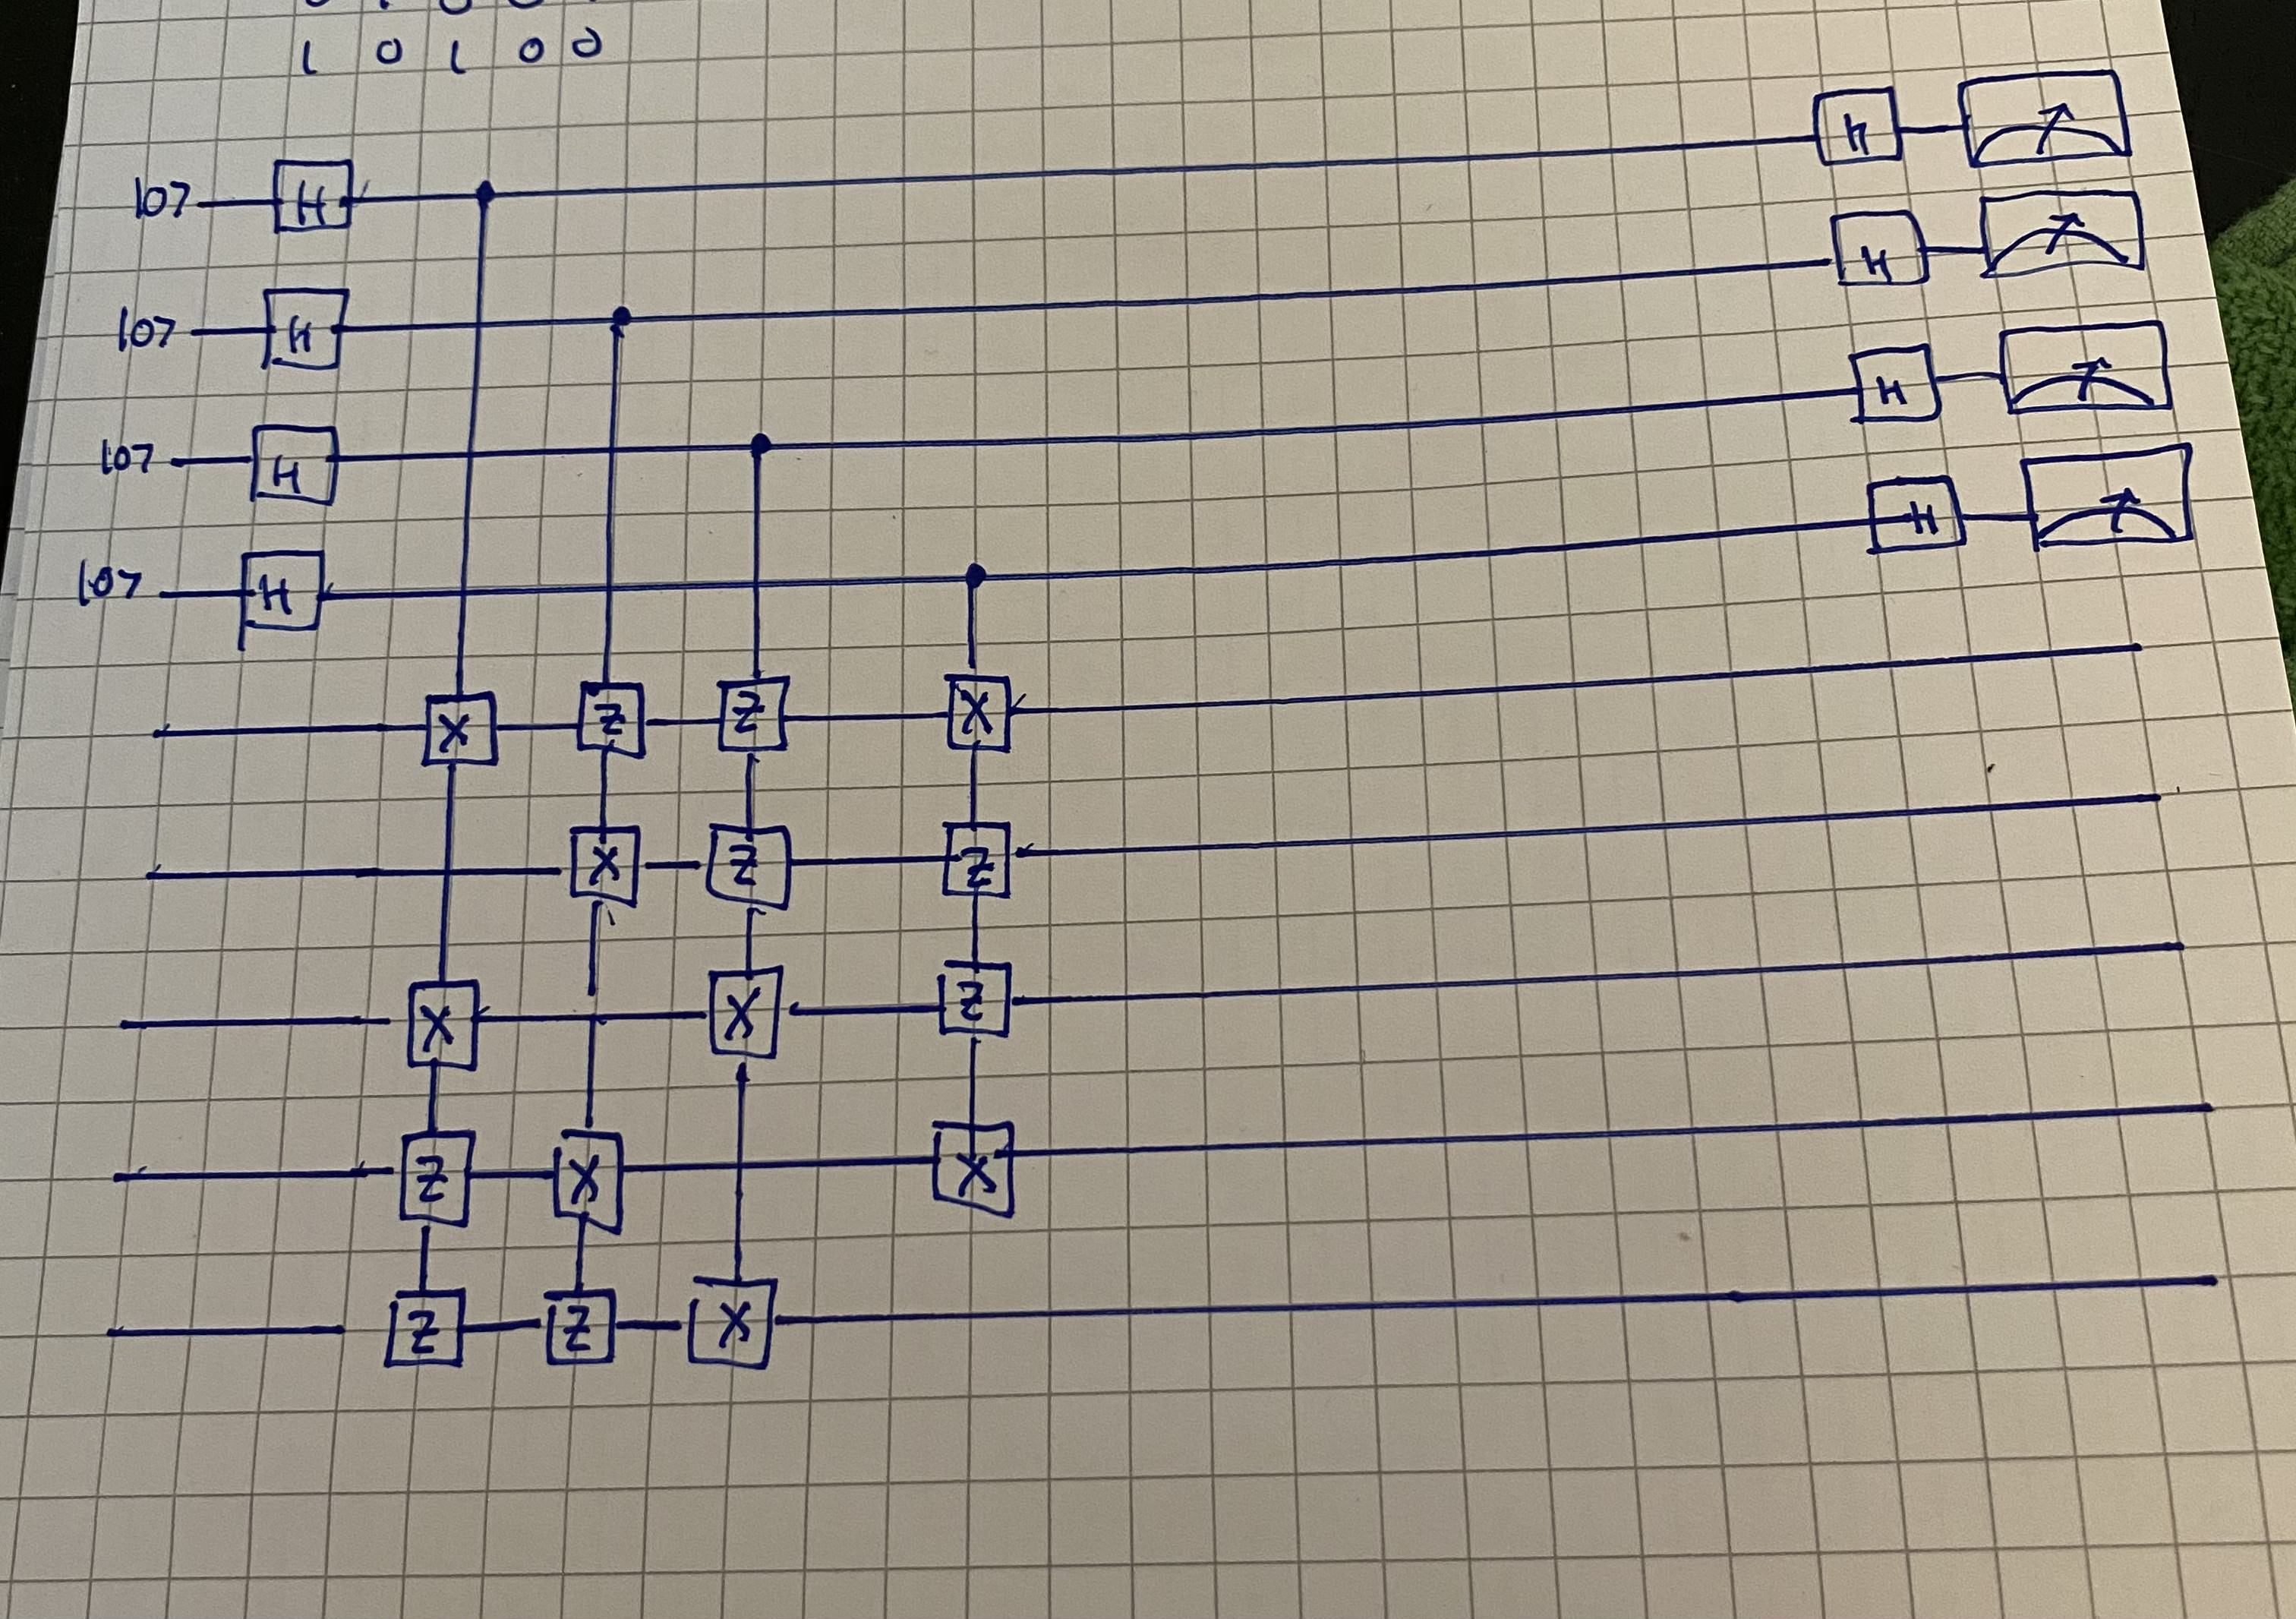
\includegraphics[width=10cm]{5qubit.jpg}
        \centering
        \caption{Syndrome measurement circuit for 5 qubit code}

    \end{figure}
    \begin{figure}[h]
        \includegraphics[width=10cm]{9qubit.jpg}
        \centering
        \caption{Syndrome measurement circuit for 9 qubit code}

    \end{figure}
\end{enumerate}




% \begin{enumerate}
%     \item Exercise 10.5. The Shor code codewords are given by 
%     $$ \ket{0} \rightarrow \ket{0_L} \equiv \frac{(\ket{000} + \ket{111}) (\ket{000}+\ket{111} )( \ket{000} +\ket{111} )}{2 \sqrt{2} } $$
%     $$ \ket{1} \rightarrow \ket{1_L} \equiv \frac{(\ket{000} - \ket{111}) (\ket{000}- \ket{111} )( \ket{000} - \ket{111} )}{2 \sqrt{2} } $$
%     If we measure observables $X_1 X_2 X_3 X_4 X_5 X_6$ and $X_4 X_5 X_6 X_7 X_8 X_9$, noticing that the last three in the first one is also the first 3 in the second part. Each 3 qubits will produce a phase flip measurement 
%     $$ \underbrace{X_1 X_2 X_3 }_{\text{1 or -1}} \underbrace{X_4 X_5 X_6 }_{\text{-1 or 1}} \equiv -1 $$
%     The $\pm 1 \ \text{or}\ \pm 1$ in the underbrace represents eigenvalues. This shows that the signs will always be different. On the other hand 
%     $$ \underbrace{X_4 X_5 X_6 }_{\text{-1 or 1}} \underbrace{X_7 X_8 X_9 }_{\text{-1 or 1}} \equiv 1 $$
%     Showing that the signs will be the same. In conclusion in this example the first 3 qubits (triplet) $X_1 X_2 X_3$ underwent a phase flip and we can correct for it. The shor code allows us to protect against bit flip or phase flip at the same time using two levels of correction instead of one. 
%     In general a phase flip or error occuring in any one of the qubits in either of the 2 6 qubit observables will change the value of either the first or last 3 qubits in the other obseravles allowing us to identify the location of the flip when measuring the observables and once identified one can correct by applying a $Z$. 
%     \\
%     \textbf{N.B}. To answer this question I tried to explain my thought process using an example situation for the shor codes.  


%     \item Exercise 10.10. The error set is 
%     $$ \{ I, X_j, Y_j, Z_j \} $$
%     For $i=1 \ldots i=9$. To satisfy the Quantum error correction conditions we have 
%     $$ P E_i E^{\dagger} E_j P = \alpha_{ij} P $$
%     For the pauli matrices this reduces to 
%     $$ P \sigma^1_i \sigma_j^1 P = \alpha_{ij} P $$
%     Even though in the book it says the calculation is quite simple I could not see it. I Do not see what the projectors onto the shor code would be
%     $$ P = \ket{0_L} \bra{0_L} + \ket{1_L} \bra{1_L} $$
%     If I could verify the projectors then I would apply the above formulae. I have seen other examples of the shor code correcting errors given by any linear combination of the pauli group, however is this what the question is asking us to show? 

    
%     \item Exercise 10.16. Adding one row to the parity check matrix does not change the code as the matrix will still span the same space. The code space is the kernel of $H$ and the kernel does not change when adding rows. Thus, Gaussian elimination and swapping of bits will give a standard form for the parity matrix. 
    
%     \item Exercise 10.19. 
%     $$ H = [A|I_{n-k}] $$
%     If $G$ is the generator matrix for the parity check matrix then 
%     $$ H G = 0 $$
%     From Ex 10.18. So 
%     $$ HG = [A|I_{n-k}] \begin{bmatrix}
%         I_k \\ \hline -A 
%     \end{bmatrix} = A-A = 0 $$
%     Therefore 
%     $$ G = \begin{bmatrix}
%         I_k \\ \hline -A 
%     \end{bmatrix} $$

%     \item Exercise 10.21. $H$ is a $n-k$ by $n$ matrix. The rank of this matrix is $n-k$. From Ex 10.20 the weight is at most $n-k +1$. Therefore, $[n,k,d]$ code satisfies $d \leq n-k +1 \equiv n-k \geq d -1$ .
    
%     \item Exerice 10.32. The 7 qubit Steane given is given by 
%     $$ H = \begin{bmatrix}
%         0&0&0&1&1&1&1 \\ 0&1&1&0&0&1&1 \\ 1&0&1&0&1&0&1 
%     \end{bmatrix} $$
%     With codewords 
%     $$ \ket{0_L} = \frac{1}{\sqrt{8}} \Big[ \ket{0000000} + \ket{1010101} + \ket{0110011} + \ket{1100110} $$
%     $$ + \ket{0001111} + \ket{1011010} + \ket{0111100} + \ket{1101001} \Big] $$
%     $$ \ket{1_L} = \frac{1}{\sqrt{8}} \Big[ \ket{1111111} + \ket{0101010} + \ket{1001100} + \ket{0011001} $$
%     $$ \ket{1110000} + \ket{0100101} + \ket{1000011} + \ket{0010110} \Big] $$
%     To make the notation easier lets make some changes 
%     $$ \ket{0000000} = \ket{a} $$
%     $$ \ket{1010101} = a_1 $$
%     $$ \ket{0110011} = a_2 $$
%     $$ \ket{0001111} = a_3 $$
%     Now notice that we can write the remaining terms for $\ket{0_L}$ as combinations of $a_1, a_2, a_3$
%     $$ \ket{1100110} = a_1 + a_2 $$
%     $$ \ket{1011010} = a_1 + a_3 $$
%     $$ \ket{0111100} = a_2 + a_3 $$
%     $$ \ket{1101001} = a_1 + a_2 + a_3 $$
%     So that 
%     $$ \ket{0_L} = \frac{1}{\sqrt{8}} \Big[ \ket{a} + a_1 + a_2 + (a_1 + a_2) + a_3 + (a_1 + a_3) + (a_2 + a_3) + (a_1 + a_2 +a_3) ] $$
%     The table from the textbook can be rewritten with 2 additional rows for $\bar{Z}$ and $\bar{X}$
%     \begin{table}[h]
%         \centering
%         \begin{tabular}{ll}
%         \hline
%         \multicolumn{1}{l|}{Name}  & Operator \\
%         \multicolumn{1}{l|}{$g_1$} & IIIXXXX  \\
%         \multicolumn{1}{l|}{$g_2$} & IXXIIXX  \\
%         \multicolumn{1}{l|}{$g_3$} & XIXIXIX  \\
%         \multicolumn{1}{l|}{$g_4$} & IIIZZZZ  \\
%         \multicolumn{1}{l|}{$g_5$} & IZZIIZZ  \\
%         \multicolumn{1}{l|}{$g_6$} & ZIZIZIZ  \\ \hline
%         $\bar{X}$                  & XXXIIII  \\
%         $\bar{Z}$                  & ZZZIIII 
%         \end{tabular}
%         \caption{Table shown in the book with two additional rows added to denote the column changes}
%         \label{tab:my-table}
%         \end{table}
%     By applying the generators $g_i$ to the codewords we see that we can get all 16 parts. Using $X: \ket{0} \rightarrow \ket{1}, \ket{1} \rightarrow \ket{0}$ and $Z: \ket{0} \rightarrow \ket{0}, \ket{1} \rightarrow \ket{-1}$.
%     $$ g_1 \ket{a} = \ket{0001111} = a_3 $$
%     $$ g_2 \ket{a} = \ket{0110011} = a_2 $$
%     $$ g_3 \ket{a} = \ket{1010101} = a_1 $$
%     $$ g_3 \ket{a} + g_2 \ket{a} = \ket{1100110} = a_1 + a_2 $$
%     $$ g_3 \ket{a} + g_1 \ket{a} = \ket{1011010} = a_1 + a_3 $$
%     $$ g_2 \ket{a} + g_1 \ket{a} = \ket{0111100} = a_2 + a_3 $$
%     $$ g_3 \ket{a} + g_2 \ket{a} + g_1 \ket{a} = \ket{1101001} = a_1 + a_2 + a_3 $$
%     The other 8 parts from $\ket{1_L}$ simply following from these noting that $\ket{1_L} = \bar{X} \ket{a}$, meaning that it is these 8 states flipped and the generators follow like before. 
% \end{enumerate}

\end{document}

